% Author: Rasmus Pank Roulund
\documentclass{standalone}
\usepackage{tikz}
\usetikzlibrary{shapes.geometric, arrows, positioning, calc, fit, arrows, decorations.pathreplacing}

\newcommand\drawcontrol[3]{%
    \draw[control] ($(#1*\xd,#2*\xd)+(xc)$) -- ++(#3);
}
\usetikzlibrary{fit,shapes.geometric}
\usetikzlibrary{
    shapes.geometric,
    decorations.pathreplacing
}
\tikzset{
    elli/.style args={#1:#2and#3}{
        draw,
        shape=ellipse,
        rotate=#1,
        minimum width=2*#2,
        minimum height=2*#3,
        outer sep=0pt,
    },
    /pgf/decoration/raise/.append code={
        \def\tikzdecorationsbrace{#1}
    },
    elli node/.style={
        circle,
        black,
        draw=none,
        midway,
        anchor=#1-90,
        inner sep=0pt,
        shift=(#1+90:\tikzdecorationsbrace+\pgfdecorationsegmentamplitude)
    }
}
\begin{document}

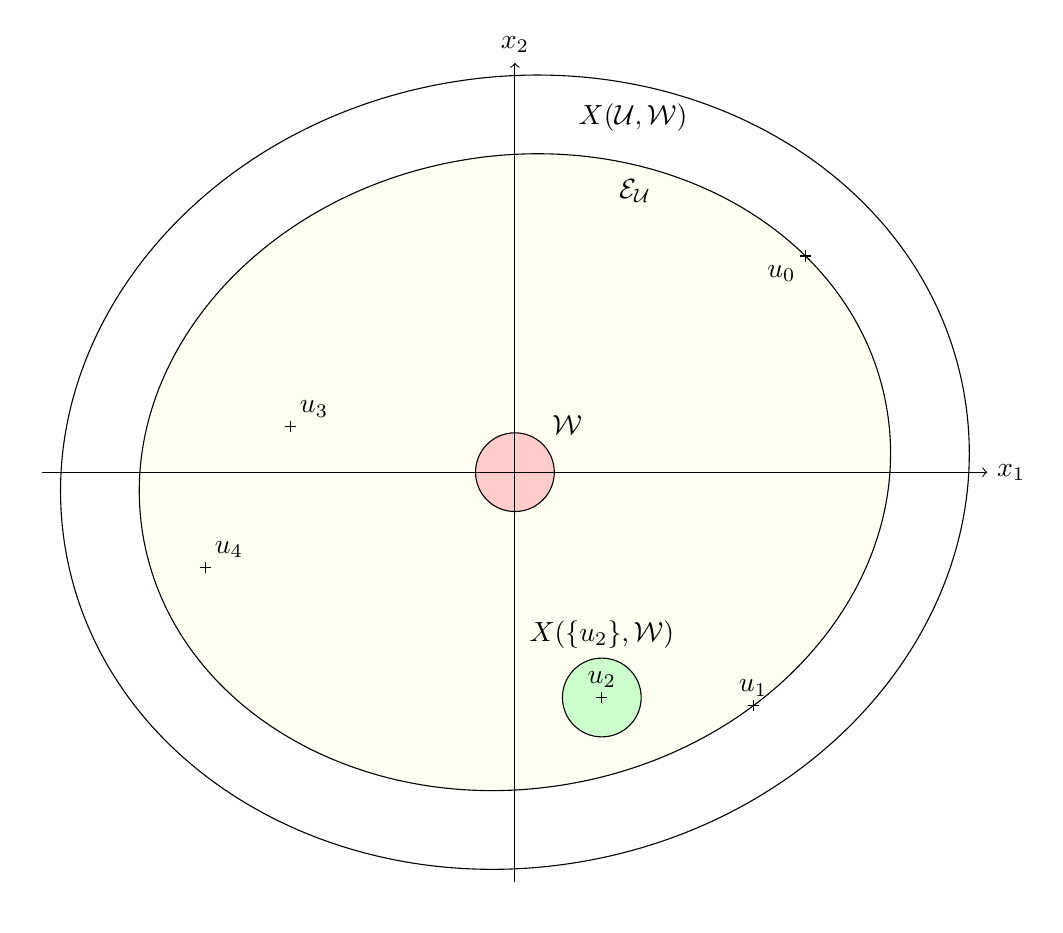
\begin{tikzpicture}



\tikzstyle{inputpoint}  = [mark=+]

\coordinate (u2) at (1.103542cm,-2.861418cm);

\node[elli=9.888353:4.791318cm and 4.018465cm,fill=yellow!05!white] at (0, 0) {};
\node[elli=0:0.5cm and 0.5cm,fill=green!20!white] at (u2) {};
\node[elli=0:0.5cm and 0.5cm,fill=red!20!white] at (0, 0) {};

\draw[->] (0,-5.2) -- (0,5.2) node (yaxis) [above] {$x_2$};
\draw[->] (-6,0) -- (6,0) node (yaxis) [right] {$x_1$};


% GENERATED WITH fit_ellipse.py
\draw[inputpoint] plot coordinates {(3.688801cm,2.745897cm)} node[anchor=north east] {$u_0$};
\draw[inputpoint] plot coordinates {(3.024680cm,-2.967980cm)} node[anchor=south ] {$u_1$};
\draw[inputpoint] plot coordinates {(1.103542cm,-2.861418cm)} node[anchor=south] {$u_2$};
\draw[inputpoint] plot coordinates {(-2.854841cm,0.575152cm)} node[anchor=south west] {$u_3$};
\draw[inputpoint] plot coordinates {(-3.935159cm,-1.208031cm)} node[anchor=south west] {$u_4$};

\node[elli=9.888353:5.791318cm and 5.018465cm] at (0, 0) {};

\node[anchor=south west] at (0.35cm,0.35cm) {$\mathcal{W}$};

\node[anchor=south] at ($(u2)+(0.cm,0.5cm)$) {$X(\{u_2\},\mathcal{W})$};

\node[anchor=south west] at (1.2cm,3.3cm) {$\mathcal{E}_\mathcal{U}$};

\node[anchor=south] at (1.5cm,4.2cm) {$X(\mathcal{U},\mathcal{W})$};

\end{tikzpicture}

\end{document}
